% {\bf A compulsory chapter,     of roughly $10$ pages} 
% \vspace{1cm} 

% \noindent
% This chapter is intended to describe the technical basis on which execution
% of the project depends.  The goal is to provide a detailed explanation of
% the specific problem at hand, and existing work that is relevant (e.g., an
% existing algorithm that you use, alternative solutions proposed, supporting
% technologies).  

% Per the same advice in the handbook, note there is a subtly difference from
% this and a full-blown literature review (or survey).  The latter might try
% to capture and organise (e.g., categorise somehow) {\em all} related work,
% potentially offering meta-analysis, whereas here the goal is simple to
% ensure the dissertation is self-contained.  Put another way, after reading 
% this chapter a non-expert reader should have obtained enough background to 
% understand what {\em you} have done (by reading subsequent sections), then 
% accurately assess your work.  You might view an additional goal as giving 
% the reader confidence that you are able to absorb, understand and clearly 
% communicate highly technical material.

As outlined in Chapter \ref{chap:context}, the objective of this project is to use deep learning to automate the calculation of the amount of skeletal matter produced by corals annually. This chapter introduces and briefly describes the techniques used in order to achieve this goal.

\section{Deep Learning}
\label{sec:deeplearning}

Based loosely on the structure of the brain, artificial neural networks (ANNs) are computational models that have proved useful in a wide range of applications~\cite{lecun2015deep, healthcare, nlp}\textemdash a notable example being the recent success of convolutional neural networks in the field of computer vision~\cite{compvision, semanticsegreview}. Deep learning is a form of machine learning that concerns the use of ANNs with many layers\textemdash hence the name ``deep'' learning. The field has seen a significant increase in popularity in recent years since a network named AlexNet famously won the ImageNet Large Scale Visual Recognition Challenge in 2012\footnote{\url{http://www.image-net.org/challenges/LSVRC/2012/results.html}}, performing considerably better than the previous state-of-the-art~\cite{alexnet}.

A typical fully connected ANN is a layered network of ``neurons'' connected by a series of ``weights''. A neuron is simply an object that produces a weighted sum of some number of inputs. This weighted sum is often passed through a non-linear ``activation'' function and the final result is referred to as the ``activation'' of the neuron. When values are supplied to the input neurons of the network, these values are forward-propagated through the network, activating each layer of neurons which, in turn, activate the next layer. The resulting activations of the neurons in the final layer are the output of the network.

\subsection{Convolutional Neural Networks}

The convolutional neural network (CNN) is a type of neural network named after the discrete convolution operation that sets these models apart from typical fully connected ANNs. The convolution operation makes use of surrounding pixels in order to change the value of a central pixel. The 2D discrete convolution operation is defined as

\begin{equation}
    g(x,y)=\sum_{i=1}^{m}\sum_{j=1}^{n}f(x-j,y-k)h(j,k)
\end{equation}

\noindent
where $f$ is the input image, $h$ is an $m\times n$ kernel, and $g$ is the resulting image.

CNNs often contain multiple convolutional layers in which increasingly complex features of an image may be detected by making use of a combination of simpler features detected in previous layers. A convolutional layer convolves the channels of an image with multiple learned kernels. A channel is simply a component of an image\textemdash an RGB image, for example, consists of three channels, whilst a greyscale image consists of only one. The output of these operations will be multiple modified images that are referred to as ``feature maps''. These feature maps can then be used as the input channels to the next layer, and so on.

As well as the convolution operation, the max-pooling operation is often used. The max-pooling operation is used to decrease the dimensionality of the input in attempt to force the network to ``learn'' features present in the input. Max-pooling layers are also used by a model to achieve some translation invariance over spatial shifts in the input image~\cite{segnet}. These operations are illustrated in Figure \ref{fig:operations}.

\begin{figure}[t]
    \centering
    \begin{subfigure}[t]{0.43\textwidth}
        \centering
        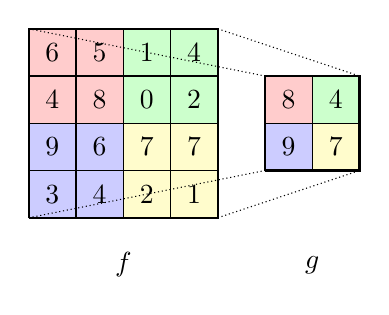
\begin{tikzpicture}[scale=0.6]
    \filldraw[color=blue, opacity=0.2] (0,0) rectangle (2,2);
    \filldraw[color=red, opacity=0.2] (0,2) rectangle (2,4);
    \filldraw[color=green, opacity=0.2] (2,2) rectangle (4,4);
    \filldraw[color=yellow, opacity=0.2] (2,0) rectangle (4,2);

    \filldraw[color=blue, opacity=0.2] (5,1) rectangle (6,2);
    \filldraw[color=red, opacity=0.2] (5,2) rectangle (6,3);
    \filldraw[color=green, opacity=0.2] (6,2) rectangle (7,3);
    \filldraw[color=yellow, opacity=0.2] (6,1) rectangle (7,2);

	\draw [thick] (0,0) -- (0,4) -- (4,4) -- (4,0) -- (0,0);
    \draw (0,1) -- (4,1);
    \draw (0,2) -- (4,2);
    \draw (0,3) -- (4,3);
    \draw (1,0) -- (1,4);
    \draw (2,0) -- (2,4);
    \draw (3,0) -- (3,4);
    \node at (0.5, 0.5) {3};
    \node at (1.5, 0.5) {4};
    \node at (2.5, 0.5) {2};
    \node at (3.5, 0.5) {1};
    \node at (0.5, 1.5) {9};
    \node at (1.5, 1.5) {6};
    \node at (2.5, 1.5) {7};
    \node at (3.5, 1.5) {7};
    \node at (0.5, 2.5) {4};
    \node at (1.5, 2.5) {8};
    \node at (2.5, 2.5) {0};
    \node at (3.5, 2.5) {2};
    \node at (0.5, 3.5) {6};
    \node at (1.5, 3.5) {5};
    \node at (2.5, 3.5) {1};
    \node at (3.5, 3.5) {4};
    
    \draw[densely dotted] (0,0) -- (5,1);
    \draw[densely dotted] (0,4) -- (5,3);
    \draw[densely dotted] (4,4) -- (7,3);
    \draw[densely dotted] (4,0) -- (7,1);
    
    \draw [thick] (5,1) -- (5,3) -- (7,3) -- (7,1) -- (5,1);
    \draw (6,1) -- (6,3);
    \draw (5,2) -- (7,2);
    
    \node at (5.5, 1.5) {9};
    \node at (6.5, 1.5) {7};
    \node at (5.5, 2.5) {8};
    \node at (6.5, 2.5) {4};
    
    \node at (2, -1) {$f$};
    \node at (6, -1) {$g$};
\end{tikzpicture}
    \vspace*{1mm}
    \caption{2D Max-pooling}
    \end{subfigure}
    ~
    \begin{subfigure}[t]{0.55\textwidth}
        \centering
        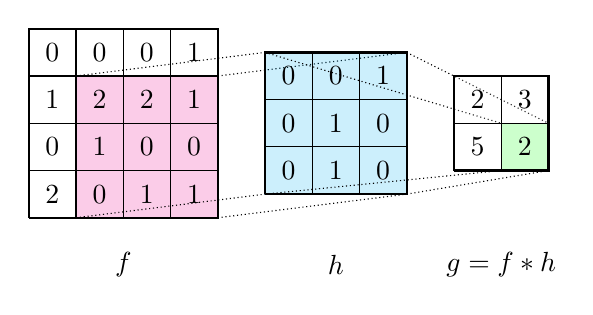
\begin{tikzpicture}[scale=0.6]
    \filldraw[color=magenta, opacity=0.2] (1,0) rectangle (4,3);

	\draw [thick] (0,0) -- (0,4) -- (4,4) -- (4,0) -- (0,0);
    \draw (0,1) -- (4,1);
    \draw (0,2) -- (4,2);
    \draw (0,3) -- (4,3);
    \draw (1,0) -- (1,4);
    \draw (2,0) -- (2,4);
    \draw (3,0) -- (3,4);
    
    \node at (0.5, 0.5) {2};
    \node at (1.5, 0.5) {0};
    \node at (2.5, 0.5) {1};
    \node at (3.5, 0.5) {1};
    \node at (0.5, 1.5) {0};
    \node at (1.5, 1.5) {1};
    \node at (2.5, 1.5) {0};
    \node at (3.5, 1.5) {0};
    \node at (0.5, 2.5) {1};
    \node at (1.5, 2.5) {2};
    \node at (2.5, 2.5) {2};
    \node at (3.5, 2.5) {1};
    \node at (0.5, 3.5) {0};
    \node at (1.5, 3.5) {0};
    \node at (2.5, 3.5) {0};
    \node at (3.5, 3.5) {1};
    
    \draw[densely dotted] (1,0) -- (5,0.5);
    \draw[densely dotted] (1,3) -- (5,3.5);
    \draw[densely dotted] (4,3) -- (8,3.5);
    \draw[densely dotted] (4,0) -- (8,0.5);
    
    \filldraw[color=cyan, opacity=0.2] (5,0.5) rectangle (8,3.5);
    
    \draw [thick] (5,0.5) -- (5,3.5) -- (8,3.5) -- (8,0.5) -- (5,0.5);
    \draw (5,2.5) -- (8,2.5);
    \draw (5,1.5) -- (8,1.5);
    \draw (6,0.5) -- (6,3.5);
    \draw (7,0.5) -- (7,3.5);
    
    \node at (5.5, 1) {0};
    \node at (6.5, 1) {1};
    \node at (7.5, 1) {0};
    \node at (5.5, 2) {0};
    \node at (6.5, 2) {1};
    \node at (7.5, 2) {0};
    \node at (5.5, 3) {0};
    \node at (6.5, 3) {0};
    \node at (7.5, 3) {1};
    
    \draw[densely dotted] (5,0.5) -- (10, 1);
    \draw[densely dotted] (5,3.5) -- (10, 2);
    \draw[densely dotted] (8,3.5) -- (11, 2);
    \draw[densely dotted] (8,0.5) -- (11, 1);
    
    \filldraw[color=white, opacity=0.2] (9,1) rectangle (10,2);
    \filldraw[color=white, opacity=0.2] (9,2) rectangle (10,3);
    \filldraw[color=green, opacity=0.2] (10,1) rectangle (11,2);
    \filldraw[color=white, opacity=0.2] (10,2) rectangle (11,3);
    
    \draw [thick] (9,1) -- (9,3) -- (11,3) -- (11,1) -- (9,1);
    \draw (10,1) -- (10,3);
    \draw (9,2) -- (11,2);
    
    \node at (9.5, 1.5) {5};
    \node at (10.5, 1.5) {2};
    \node at (9.5, 2.5) {2};
    \node at (10.5, 2.5) {3};
    
    \node at (2, -1) {$f$};
    \node at (6.5, -1) {$h$};
    \node at (10, -1) {$g=f\ast h$};
\end{tikzpicture}
        \vspace*{1mm}
        \caption{2D Convolution}
    \end{subfigure}
    \caption{Illustrations of the 2D max-pooling and convolution operations. \textbf{(a)} The max-pooling operation shown takes an input image $f$ and uses a 2$\times$2 filter and stride of two to produce the output image $g$. Note that the maximum value in each coloured region of the input is the resulting value of the corresponding regions of the output. \textbf{(b)} The convolution operation shown takes an input image $f$ and uses a 3$\times$3 kernel $h$ with a stride of one to produce the output image $g=f\ast h$, where $\ast$ denotes the convolution operation. Note that the kernel shown in the convolution operation is ``flipped'' in both the $x$ and $y$ axes before the element-wise multiplication and summation takes place.}
    \label{fig:operations}
\end{figure}

Another feature of CNNs that set them apart from their fully connected counterparts is the localised ``receptive fields'' of the neurons present in convolutional layers. Whilst neurons present in a fully connected layer can receive input from every neuron in the previous layer, neurons present in a convolutional layer can only receive input from a small amount of neighbouring neurons in the previous layer. For example, if a 3$\times$3 kernel is used, a neuron's activation can only be influenced by nine neurons in the previous layer. This area of input that can influence a neuron is called its receptive field. This is one of the reasons why during hyper parameter optimisation, kernel sizes from various layers may be tuned in order to increase or decrease the size of neurons' receptive fields. Hyper parameter optimisation is discussed in Section \ref{sec:hyperparam}.

\subsection{Backpropagation}
\label{sec:backprop}

First popularised by Rumelhart et al. in 1986~\cite{rumelhart}, the backpropagation algorithm is still the main learning mechanism used in neural networks today. Once a loss function is defined to measure the performance of the network, backpropagation can be used to compute the derivative of the loss function with respect to each weight in the network using the chain rule. The derivatives are calculated one layer at a time, iterating backward from the output layer. Since the backpropagation algorithm makes use of the chain rule, the loss function must be differentiable. This must also be the case for the chosen activation functions for each neuron.

An optimisation algorithm can then use these computed derivatives to adjust each weight in order to minimise the chosen loss function. Loss functions used throughout this project are discussed in Section \ref{sec:loss}.

\subsection{Optimisation Algorithms}

Once the derivatives\textemdash or ``gradients''\textemdash have been calculated, an optimisation algorithm is used to determine the exact value each weight should be updated to. When training deep neural networks, some variant of the gradient descent algorithm is often used. Gradient descent~\cite[p. 536]{gradient} is an iterative algorithm designed to find local minima of some differentiable function\textemdash in this case, the loss function. A visualisation of the gradient descent algorithm is shown in Figure \ref{fig:gd}. The gradient descent algorithm evaluates the loss function over the entire dataset before taking a ``step'' in the direction of the gradient computed. A step consists of updating the value of every weight in order to decrease the average loss value that would be achieved by the network when processing the dataset. Evaluating the loss function over the entire dataset once is referred to as an ``epoch''.

The size of the weight update is not only determined by the gradient calculated, but also by a hyper parameter called the ``learning rate''. For example, gradient descent calculates the update for a single weight $w$ as

\begin{equation}
    w := w - \eta\nabla\ell(w)
\end{equation}

\noindent
where $\eta$ is the learning rate and $\nabla\ell(w)$ is the derivative of the loss function $\ell$ with respect to $w$. Choosing an appropriate learning rate is challenging but is essential to allow an optimisation algorithm to converge to a local minimum. A learning rate that is too large can cause the loss function to fluctuate around the minimum, impeding convergence or even causing divergence. The learning rate hyper parameter has a significant effect on training and is one of the most important parameters tuned in the hyper parameter optimisation process (see Section \ref{sec:hyperparam}).


\subsubsection{Stochastic Gradient Descent}

Issues arise when using gradient descent with larger datasets, as evaluating the loss function over the entire dataset before a step can be taken becomes increasingly computationally costly~\cite{gdbad}. These issues have given rise to the popularity of the stochastic gradient descent (SGD) and the mini-batch gradient descent optimisation algorithms. SGD is a variant of the gradient descent algorithm that takes a step each time a sample is processed rather than only once the entire dataset is processed. Mini-batch gradient descent is yet another variant of gradient descent in which weights are updated after evaluating the loss function over a subset\textemdash or ``batch''\textemdash of the training samples.

\begin{figure}[t]
    \centering
    \begin{tikzpicture}[scale=1.1]
	\begin{axis}[
% 	colormap/greenyellow,
	colormap name=cool2,
% 	view={0}{90}
	xlabel=$x$,
	ylabel=$y$,
	zlabel=Loss,
	zmin=0.1, zmax=1.9,
	xtick distance=175,
	ytick distance=175,
	xticklabels=\empty,
	yticklabels=\empty,
	zticklabels=\empty
	]
% 	\addplot3[surf,
% 		domain=0:360,samples=40] 
% 		{0.5*sin(x-100)*sin(y-50) - 0.000005*((x-100)^2) + 0.000005*((y-50)^2) + 1};
    \addplot3 [surf, mesh/rows=36] table [x=xs, y=ys, z=zs, col sep=comma] {csv/surf.csv};
    
	\addplot3 [black, mark=*, line width=0.8pt, mark size=0.8pt] table [x=xs, y=ys, z=zs, col sep=comma] {csv/sgd.csv};
	
	\addplot3 [black, mark=*, line width=0.8pt, mark size=0.8pt] table [x=xs, y=ys, z=zs, col sep=comma] {csv/sgd3.csv};
	
	\node[] at (axis cs: 320, 200, 1.9) {\scriptsize{($x_0, y_0, \ell(x_0, y_0)$)}};
	
	\node[] at (axis cs: 260, 200, 0.1) {\scriptsize{($x_n, y_n, \ell(x_n, y_n)$)}};
	\end{axis}
\end{tikzpicture}
    \caption{A diagram visualising the gradient descent algorithm for a model containing two trainable parameters, $x$ and $y$. Given a random starting configuration with parameters $x_0$ and $y_0$, the average loss value that would be achieved when processing the entire dataset is given by $\ell(x_0, y_0)$. Say gradient descent takes $n$ steps in the direction of steepest descent at each iteration until the loss value converges to some local minimum, $x_n$ and $y_n$ would be the final parameter values and the final loss would be $\ell(x_n, y_n)$. It is worth noting that even though the two starting configurations shown in the diagram both converge to the same local minimum, this might not always be the case. A starting configuration nearer to one of the other possible local minima would most likely not converge to the example local minimum $\ell(x_n, y_n)$ shown.}
    \label{fig:gd}
\end{figure}

\subsubsection{Adam}

First introduced by Kingma and Ba in 2014, Adam~\cite{adam} is an optimisation algorithm that is also based off of SGD. However, rather than using the same learning rate across all parameters, Adam computes individual adaptive learning rates for different parameters. These individual learning rates are based off of estimates of the first moment (the mean) and second moment (the uncentered variance) of the gradients~\cite{gdbad}. Kingma and Ba showed empirically that Adam works well in practice and compares favourably to other optimisation algorithms when optimising both fully connected ANNs and deep CNNs.

\subsection{Loss functions}
\label{sec:loss}

A loss function takes both the actual and predicted values of a training sample, and outputs some measure of how well a model performed by producing that prediction. As mentioned in Section \ref{sec:backprop}, backpropagation makes use of the derivative of the loss function with respect to each parameter in order to minimise the loss achieved. If the appropriate loss function is chosen, minimising the loss should improve the performance achieved by the network. It is for this reason that loss functions must be differentiable. The loss functions that were experimented with throughout this project are outlined below.

\subsubsection{Binary Cross-Entropy Loss}

The binary cross-entropy loss function is used when classifying samples that can belong to two classes. When performing image classification, a model will produce two probabilities\textemdash one for each class. When performing image segmentation, a model effectively classifies each pixel; thus, two probabilities will be produced for each pixel. These are the model's predicted probabilities that a given image (or pixel) belongs to each of the two classes. Since these two classes are the only possible classes that the model can predict, the probabilities should sum to one. The binary cross-entropy loss is defined as:

\begin{equation}
    CE(p, y) = 
    \begin{cases}
        -\log(p) & \text{if } y = 1\\
        -\log(1 - p) & \text{otherwise}
    \end{cases}
\end{equation}

where $y \in \{+1, -1\}$ is the actual value (the ground-truth), and $p \in [0, 1]$ is the model's estimated probability for the class with label $y = 1$. This is the loss value achieved when classifying a single training sample.

\subsubsection{Binary Focal Loss}

Proposed by Lin et al. in 2018, the Focal Loss~\cite{focalloss} is designed to address the ``class imbalance'' problem. In a typical classification problem, class imbalance occurs when one class contains significantly fewer samples than the other classes. Lin et al. highlight the fact that when using the cross-entropy loss function, even samples that are well-classified incur a loss with ``non-trivial'' magnitude. When summed over large numbers of samples from the easily classified majority class, these small loss values can overwhelm the loss resulting from the minority class samples~\cite{focalloss}.

In an attempt to address this problem, the focal loss introduces two new parameters: a weighting factor $\alpha \in [0, 1]$ and a ``focusing'' parameter $\gamma \geq 0$.
The binary focal loss is then defined as:

\begin{equation}
    \text{FL}(p, y) = 
    \begin{cases}
        -\alpha(1 - p)^{\gamma} \log (p) & \text{if } y = 1\\
        (1 - \alpha)p^{\gamma} \log (1 - p) & \text{otherwise}
    \end{cases}
\end{equation}

where $y \in \{+1, -1\}$ is the actual value (the ground-truth), and $p \in [0, 1]$ is the model's estimated probability for the class with label $y = 1$. The weighting factor increases the loss produced by the misclassification of minority class samples whilst the focusing factor ``reduces the contribution from easy examples and extends the range in which an example receives low loss''~\cite{focalloss}. When $\gamma = 0$ and $\alpha = 1$, the focal loss is equivalent to the cross-entropy loss. The contribution of the $\gamma$ value to the loss produced can be seen in Figure \ref{fig:focal}.

\begin{figure}[t]
    \centering
    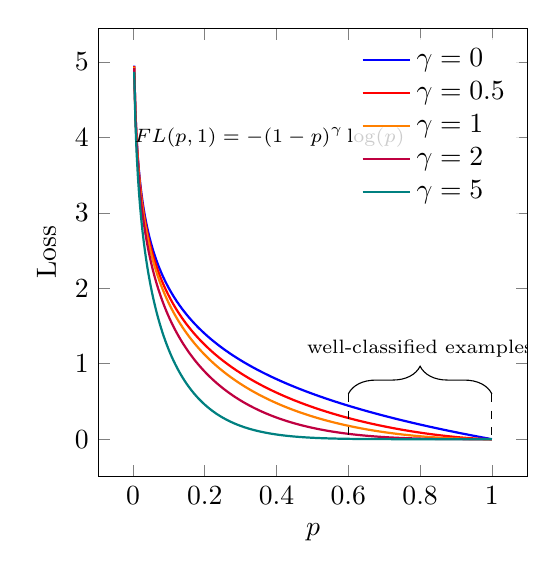
\begin{tikzpicture}
	\begin{axis}[
		xlabel=$p$,
		ylabel=Loss,
		width=0.58\textwidth,
        height=\axisdefaultheight,
        legend cell align=left,
        legend style={fill=white, fill opacity=0.8, draw=none,text opacity=1}
	]
	
	\addplot[samples=300, domain=0:1, thick, blue]   {2 * -(1-x)^0   * log10(x)};
	\addlegendentry{$\gamma = 0$}
	\addplot[samples=300, domain=0:1, thick, red]    {2 * -(1-x)^0.5 * log10(x)};
	\addlegendentry{$\gamma = 0.5$}
	\addplot[samples=300, domain=0:1, thick, orange] {2 * -(1-x)^1   * log10(x)};
	\addlegendentry{$\gamma = 1$}
	\addplot[samples=300, domain=0:1, thick, purple] {2 * -(1-x)^2   * log10(x)};
	\addlegendentry{$\gamma = 2$}
	\addplot[samples=300, domain=0:1, thick, teal]   {2 * -(1-x)^5   * log10(x)};
	\addlegendentry{$\gamma = 5$}
	
	\node[] at (0.38, 4) {\scriptsize{$\text{FL}(p, 1) = -(1 - p)^{\gamma} \log (p)$}};
	\draw [decorate,decoration={brace,amplitude=10pt}]
	(0.6, 0.6) -- (1, 0.6) node[midway]{};
	\node[] at (0.8, 1.2) {\scriptsize{well-classified examples}};
	\draw[dashed] (0.6, 0.6) -- (0.6, 0);
	\draw[dashed] (1, 0.6) -- (1, 0);
	\end{axis}
\end{tikzpicture}
    \caption{An illustration of the focal loss with varying values of $\gamma$. Recreated from \cite{focalloss}: ``setting $\gamma > 0$ reduces the relative loss for well-classified examples $(p > 0.5)$, putting more focus on hard, misclassified examples''.}
    \label{fig:focal}
\end{figure}

\subsection{Accuracy Metrics}

Although loss functions can be used to measure performance, their main purpose is to be used to train the network. To quantify the performance achieved by a network, an accuracy metric should instead be used. Accuracy metrics do not play a direct role in training networks, though they can be used indirectly\textemdash for example, to determine whether or not to continue training. Choosing an appropriate accuracy metric is essential and proved challenging throughout this project. The main accuracy metric decided upon was based off of the Hausdorff distance discussed in Section \ref{sec:hausdorff}.

\subsection{Overfitting and Regularization}

The term overfitting refers to the phenomenon when a model performs well on the data on which it is trained, yet poorly on data which it has not yet been exposed to. Overfitting is still a serious problem faced whilst training deep networks due to the large amount of parameters that must be learned~\cite{dropout, reducing, overfitavoid}. Regularization is any technique that is used in order to reduce overfitting and allow a model to generalise better~\cite{regular}. This section introduces some of the regularization techniques used throughout the project.

\subsubsection{Data augmentation}

A very common technique used to reduce overfitting is data augmentation. Data augmentation is the process of augmenting the labelled training data in some way in order to increase the amount of training data available. This augmentation can be performed ``online'' with each training sample being randomly augmented during the training process, or it can be performed ``offline'' with the augmentation taking place before training. The training data can be augmented in many ways. Common examples for 2D images are: random rotations within some predefined range, random changes to brightness levels, and random horizontal and vertical flips. Effective data augmentation allows for a dataset to be artificially expanded, enabling it to represent a more comprehensive set of possible samples.

\subsubsection{Dropout}

Another technique often used to reduce overfitting is dropout. The use of dropout as a regularization technique when training neural networks was first popularised by Srivastava et al.~\cite{dropout} in 2014. Throughout the training process, subsets of randomly selected neurons (and their connections) are ``dropped''. Only the resulting reduced network is then trained on a particular training sample. A subset of dropped neurons will only remain dropped whilst processing a single training sample; the dropped neurons will then be added back to the network and a different subset of neurons will be dropped when processing the next training sample. The choice of which subset of neurons to drop for each training sample is random. 

Dropout reduces overfitting by preventing neurons from ``co-adapting'' too much~\cite{dropout}. Co-adaptation between neurons refers to the phenomenon when one neuron relies too heavily on the input from another neuron. If one neuron relies too heavily on the input of another neuron, the receiving neuron's performance in producing an activation that would be beneficial to the performance of the network may be hindered by the one ``bad'' input\textemdash even if the inputs from all other incoming neurons were ``good''.

\subsubsection{Cross-Validation}

When training and evaluating a model, the dataset is often split into three subsets: the training set, the validation set, and the test set. The training set is often the biggest subset and is used to fit the model. This is the set that the model ``learns'' from. The validation set is used to provide an unbiased evaluation of the model's performance on the dataset which can then be used to tune hyperparameters (discussed in Section \ref{sec:hyperparam}). Note that the evaluation of the models performance provided by the validation set becomes more biased each time the validation performance is used to tune hyperparameters. It is important to keep the training and validation sets separate; the model must not be directly trained on any validation data. The test set is used to provide an unbiased evaluation of the final model. The test set is only used once the final model hyperparameters are chosen and the model has been trained. Evaluating the model's performance on a single test set may not be robust to ``selection biases''\textemdash biases that arise from selecting a particular test set. Although curating a test set that represents a wide range of possible data samples can help reduce selection bias, some amount of bias is still inevitable.

In order to reduce the effects of selection bias, a cross-validation technique can be used. Cross-validation is designed to give a comprehensive measure of a model's performance throughout the entire dataset, not just a particular subset.  Once the model's hyperparameters and training configuration have been finalised, multiple train/test splits can be used. For each new train/test split, the model can be re-trained and its performance will be evaluated on the new test set. This process can be repeated with multiple random train/test splits and the final reported performance will be the average of the performances achieved on each test set. In order to ensure that the final performance achieved is not biased, it is important to ensure that the model and its hyperparameters are not modified during the cross-validation process.

\subsubsection{Early Stopping}
Referred to as a ``beautiful free lunch'' by Geoffrey Hinton~\cite[p. 141]{earlystoppinglunch}, early stopping is a regularization technique in which the training process is stopped given some ``stopping criteria'' rather than after a set number of epochs. The simplest stopping criteria is to stop training as soon as the loss achieved on the validation set increases after an epoch rather than decreases. However, when training complex models, the ``loss curve'' achieved on the validation set may contain many local minima~\cite{earlystopping}. A more common method is to stop training once the loss achieved on the validation set fails to decrease after a certain number of epochs. This method helps to prevent noise in the validation loss curve from stopping the training process prematurely. A simple example of early stopping for an ideal loss curve is shown in Figure \ref{fig:earlystop}.

\begin{figure}[t]
    \centering
    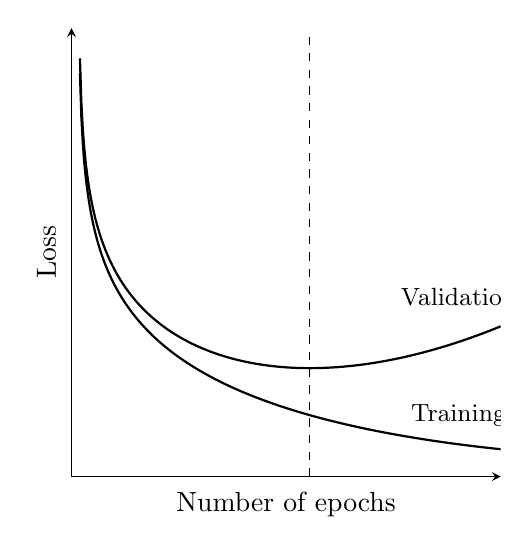
\begin{tikzpicture}
	\begin{axis}[
		xlabel=Number of epochs,
		ylabel=Loss,
		width=0.58\textwidth,
        height=\axisdefaultheight,
        axis x line=bottom,
        axis y line=left,
        % axis lines*=left,
        ymin=-0.1,
        ymax=3,
        xmin=-0.05,
        xmax=3,
        xtick=\empty,
	    ytick=\empty,
	]

	\addplot[samples=300, domain=0:3, thick, black]   {-(1 - x / 5) * log10(x / 5)};
	\addplot[samples=300, domain=0:3, thick, black]    {-(1 - x / 5) * log10(x / 5) + (x^2) / 12 + 0.1};

	\node[] at (2.7, 1.14) {\small{Validation}};
	\node[] at (2.7, 0.32) {\small{Training}};
	\draw[dashed] (1.64, -0.1) -- (1.64, 3);
	\end{axis}
\end{tikzpicture}
    \caption{An illustration of idealised training and validation loss curves. Both the training and validation loss decrease until a point. However, from this point onward, although the training loss continues to decrease, the validation loss begins to increase and the model begins to overfit. This point at which the validation is lowest is the ideal time to stop the training process.}
    \label{fig:earlystop}
\end{figure}

\subsection{Ablation Studies}

\subsection{Hyper parameter optimisation}
\label{sec:hyperparam}

Define what a parameter and hyper parameter is. Talk about diff algorithms (genetic vs brute force).

\section{Network Architectures}

Various CNN architectures are experimented with throughout this project. This section introduces and details these architectures.

\subsection{SegNet}

In 2015, Badrinarayanan, Kendall, and Cipolla~\cite{segnet} introduced SegNet: a fully convolutional neural network architecture for semantic pixel-wise segmentation that was primarily motivated by road scene understanding applications. An architecture is ``fully convolutional'' when it contains no fully connected layers. The architecture consists of an ``encoder'' and a ``decoder'' with some extra pass through of information from layers early in the encoder to later layers in the decoder.

An encoder is a model or part of a model that takes some input and ``encodes'' the input into some lower dimensional representation. For example, a typical CNN architecture used for image classification is an example of an encoder since the input could be some high resolution two dimensional image and the output would be a small number of probabilities\textemdash one for each possible class that the image could be classified as. In fact, the encoder architecture used in SegNet is topologically identical to the convolutional layers used in the VGG16 architecture used for image classification~\cite{segnet, vgg16}. A decoder can be thought of as the opposite of an encoder; given some input, a decoder will ``decode'' the input back into some higher dimensional representation.

% The encoder consists of five blocks each containing multiple 3$\times$3 convolutional layers followed by a 2$\times$2 max-pooling layer. The decoder also consists of five of blocks, however, each block contains a 2$\times$2 upsample layer followed by multiple 3$\times$3 convolutional layers. The output of each convolutional layer is passed through a ReLU activation function.

The information passed through from the encoder to the decoder is in the form of max-pooling ``indices''. The decoder uses pooling indices computed in the max-pooling step of corresponding encoder layers to perform non-linear upsampling. These indices are simply the locations of the maximum value in each pooling window. This approach eliminates the need for the architecture to ``learn'' the indices to use to upsample with since the indices that it will use are already learned in the max-pooling layers of the encoder.

\subsection{U-Net}

Presented by Ronneberger et al. in 2015~\cite{ronneberger2015u}, U-Net is a convolutional neural network architecture that was initially used to perform image segmentation on biomedical images, but has since been used on a wider range of visual data. At a high level, the U-Net architecture consists of three sections: the contracting path, the bottleneck, and the expanding path. The contracting path follows the typical architecture of a convolutional network, in that the image is gradually downsampled via convolutional and max-pooling layers and the number of feature channels is increased. The expansion path then gradually reconstructs the image via `up-convolutions'. Throughout the expansion path, the feature channels from the corresponding contraction layers are appended to the feature channels in the expansion layers. This allows the features that are learned whilst contracting the image to also be used to reconstruct it. A diagram of the U-Net architecture is shown in Figure~\ref{fig:unet}.

The U-Net and SegNet architectures share multiple similarities. They are both fully convolutional architectures designed to perform semantic pixel-wise segmentation. Both architectures also consist of an encoder, a bottleneck, and a decoder, with the encoder following a typical CNN architecture. Note that when describing the U-Net architecture, Ronneberger et al. refer to the encoder and decoder as the contracting and expanding paths respectively. Another similarity between the architectures is their passing of information from layers in the encoder to corresponding layers in the decoder. However, the passing of information is implemented differently in each architecture. Whilst U-Net passes information by concatenating feature maps from layers in the encoder to the feature maps of layers in the decoder, SegNet passes information in the form of pooling indices.

\begin{figure}[t]
    \centering
    \begin{tikzpicture}[scale=0.4]
    \node[above] at (13, 3) {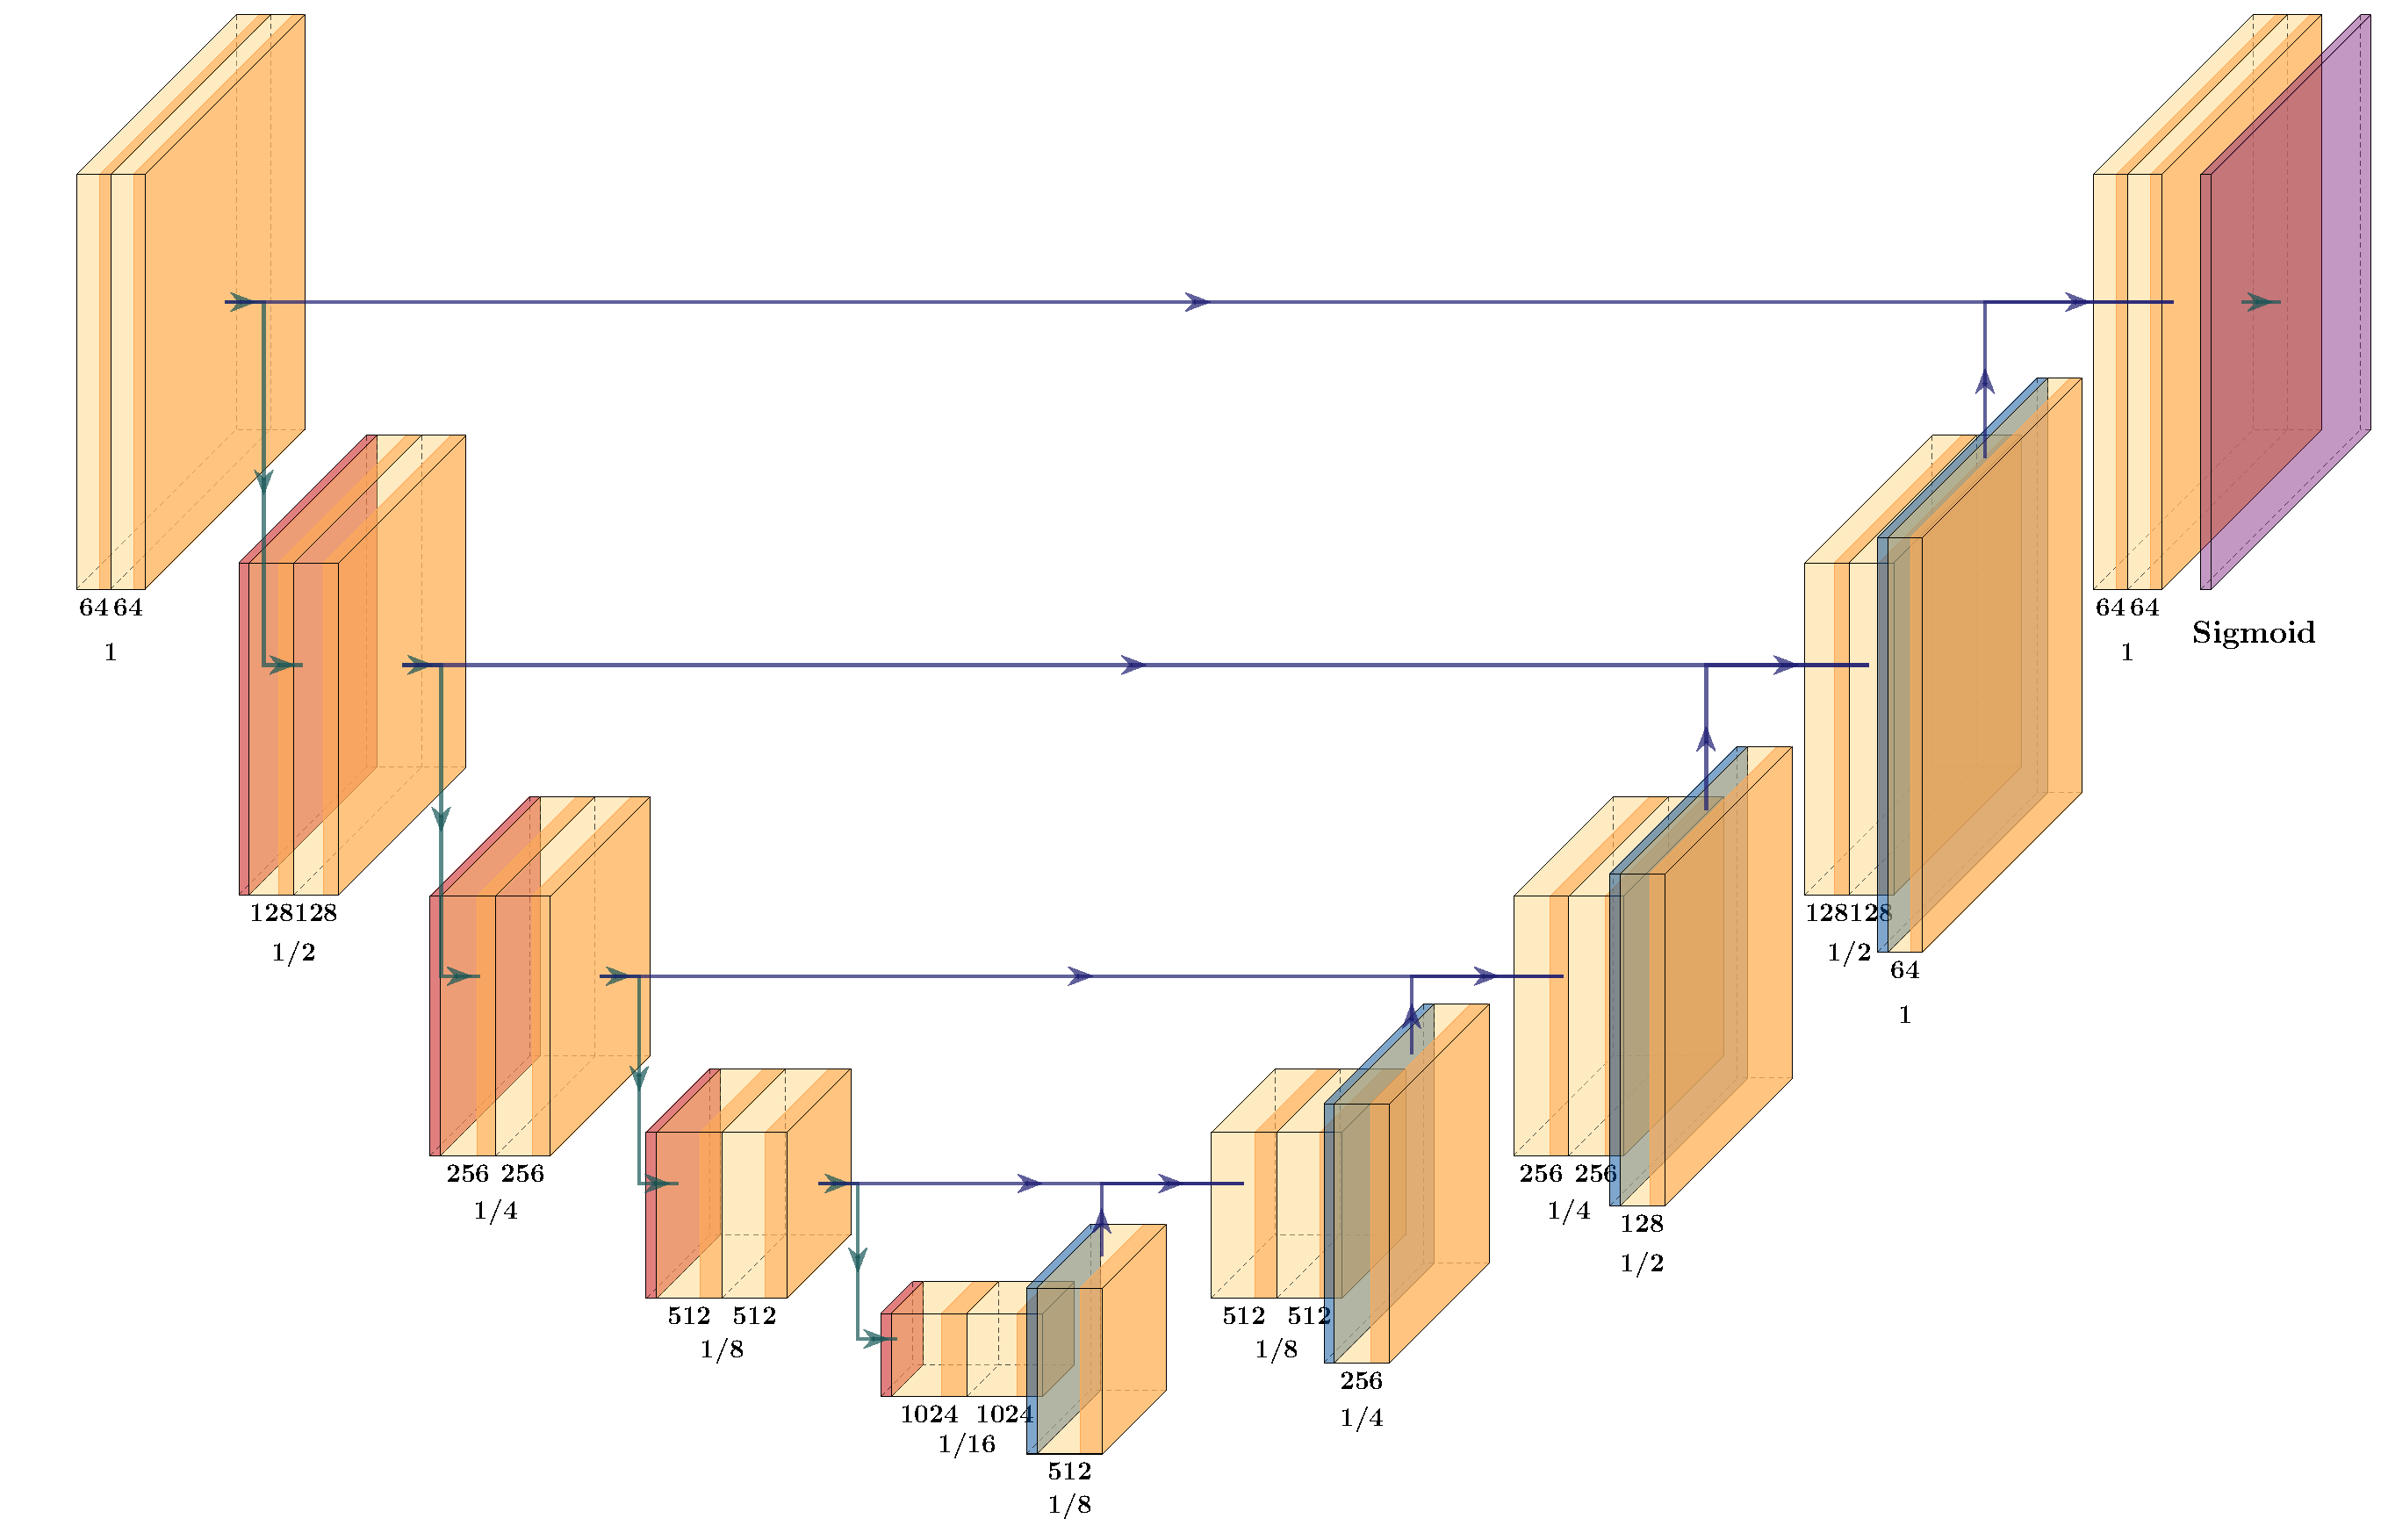
\includegraphics[width=1\textwidth]{images/U-Net.pdf}};
    
    \filldraw[color=\ConvColor, opacity=0.5] (0,1.5) rectangle (1,2.5);
    \draw[] (0,1.5) rectangle (1,2.5);
    \node[right] at (1, 2) {\scriptsize{3$\times$3 Convolution}};
    
    \filldraw[color=\ConvReluColor, opacity=0.8] (0,0) rectangle (1,1);
    \draw[] (0,0) rectangle (1,1);
    \node[right] at (1, 0.5) {\scriptsize{ReLU}};
    
    \filldraw[color=\PoolColor, opacity=0.75] (9,0) rectangle (10,1);
    \draw[] (9,0) rectangle (10,1);
    \node[right] at (10, 0.5) {\scriptsize{2$\times$2 Max-pooling}};
    
    \filldraw[color=\UnpoolColor, opacity=0.7] (9,1.5) rectangle (10,2.5);
    \draw[] (9,1.5) rectangle (10,2.5);
    \node[right] at (10, 2) {\scriptsize{2$\times$2 Up-convolution}};
    
    % \filldraw[color=\PoolColor, opacity=1] (18,0) rectangle (19,1);
    % \draw[] (18,0) rectangle (19,1);
    \node[right] at (19, 0.5) {\scriptsize{Feedforward}};
    
    % \filldraw[color=\PoolColor, opacity=1] (18,1.5) rectangle (19,2.5);
    % \draw[] (18,1.5) rectangle (19,2.5);
    \node[right] at (19, 2) {\scriptsize{Concatenation}};

    \begin{scope}[decoration={
        markings, mark=at position 0.75 with {\arrow[scale=1.5]{stealth}}}] 
        \draw[postaction={decorate}, color={rgb:blue,4;red,1;green,4;black,3}] (18,0.5)--(19,0.5);
        \draw[postaction={decorate}, color={rgb:blue,4;red,1;green,1;black,3}] (18,2)--(19,2);
    \end{scope}
\end{tikzpicture}
    \caption{A diagram of the U-Net architecture. Each cube represents a layer with the number of output feature maps shown at the bottom of the cube. At the bottleneck there are 1024 feature maps that are each one sixteenth the size of the input image in the $x$ and $y$ dimensions. The green arrows represent the feedforward of information from one layer to the next, whereas the blue arrows represent the concatenation of the feature maps of one layer to another.}
    \label{fig:unet}
\end{figure}

\subsection{Generative Adversarial Networks}

A generative adversarial network (GAN)~\cite{gans} is a framework in which two models are pitted against each other: a generative model $G$ that captures the data distribution and a discriminative model $D$ that estimates the probability that a sample came from the training data rather than $G$. Both are models are trained simultaneously, and in competition with each other. The training procedure for $G$ is to maximize the probability of $D$ making a mistake.

Many problems in image processing and computer vision involve ``image-to-image translation'': the translation of an input image into some corresponding output image. In recent years, adversarial nets have proved to be an effective general-purpose solution to image-to-image translation~\cite{gansoverview}. For example, the pix2pix model~\cite{pix2pix} demonstrates effective results in different computer vision tasks that had previously required special purpose models, including semantic segmentation and colorisation of black and white images.

\section{Classical Image Processing Techniques}

\subsection{Hausdorff distance}
\label{sec:hausdorff}

\begin{figure}[h]
    \centering
    \includegraphics[width=0.45\textwidth]{example-image-a}
    \caption{Hausdorff illustration}
    \label{fig:hausdorff}
\end{figure}

\section{Supporting Technologies}

\subsection{Keras}

The Keras\footnote{\url{https://keras.io}} library is used to implement all architectures experimented with throughout this project. Keras is an open-source library written in Python that can be used to build and train deep learning models. Keras is capable of running on top of the TensorFlow\footnote{\url{https://tensorflow.org}} library allowing code to be run on both CPUs and GPUs.

Keras offers two APIs that can be used to define a model architecture: the sequential API\footnote{\url{https://keras.io/getting-started/sequential-model-guide}} and the functional API\footnote{\url{https://keras.io/getting-started/functional-api-guide}}. The sequential API is easier to use and allows users to define a model architecture by simply passing a list of layer instances to the sequential constructor. However, the sequential API is limited in that it does not allow users to define architectures that share layers or have multiple inputs or outputs. Since the architectures implemented throughout this project contain layers that take inputs from more than one previous layer, the functional API must be used.

A simple example of how to define and train a model architecture using the Keras library is shown in Listing \ref{lst:one}.

\begin{lstlisting}[float={ht},caption={An small code snippet defining a simple model with an input of a 1D tensor of length 784, two hidden layers both containing 64 units with ReLU actiation functions, and an output layer containing 10 units using the softmax activation function.},label={lst:one},language=Python,upquote=true]
from keras.layers import Input, Dense
from keras.models import Model
from keras.optimizers import Adam

# Define the input layer
inputs = Input(shape=(784,))

# Define the hidden and output layers
linear1 = Dense(64, activation='relu')(input)
linear2 = Dense(64, activation='relu')(linear1)
outputs = Dense(10, activation='softmax')(linear2)

# Create the model
model = Model(inputs=inputs, outputs=outputs)

# Compile the model
model.compile(optimizer=Adam(lr = 1e-4),
              loss='categorical_crossentropy',
              metrics=['accuracy'])

# Train the model on labelled data
model.fit(data, labels)
\end{lstlisting}